\section{Class diagram}

\todo[inline]{Relire, mélange de noms des classes en anglais et français?}

The following class diagram is a schematic representation of the various
objects used in our implementation and their relations. In this section we will
give a short explanation of each class, and their utility in the application.\newline

First, the \textit{Participant} class is used to represent a player in the
application. Once an account as been created on the website, an instance
of the \textit{Participant} class will be created, which will store all
the data of the player. This class also extends the default \textit{User} class
of Django, which is appropriate to safely store passwords and usernames in
the database through built-in encryption.\newline

If a player has not yet validated his mail address, an instance of
\textit{UserInWaitOfActivation} class will also be created. This object
contains the key which will allow the player to validate his or her email
address, as well as set the date for the account creation. If an
account has not been validated for more than seven days it will automatically
be deleted, as it will surely never be validated in the future.\newline

For staff members, which are also represented as instances of the
\textit{Participant} class, the \textit{LogActivity} class will also be used
to store the data of some operations they can perform on the website. \newline

Similarly to the \textit{Participant} class, the \textit{Court} class is used
to represent courts, and to contain the corresponding information.
As you can see, both classes holds a latitude and longitude attribute,
allowing us to store their emplacement on a map tool, such as Google Maps.
That information can then be used to reduce participant's travel distance
during the tournament creation, by selecting a court that is the closest to
all the participants of the group. \newline

As you can see the \textit{Court} class is also linked to three small classes,
\textit{CourtSurface}, \textit{CourtState} and \textit{CourtType}, which serve
to alleviate the load on the database by reducing data replication.
The \textit{Participant} class is similarly linked to a small \textit{Ranking}
class which serve the same purpose. \newline

The \textit{Pair} class is used to store the data of a pair in the application.
Each pair is composed of two participants and various other attributes, such
as the list of extras that they chooses to pay for (through the
\textit{Extra} class), or if they have already payed at all. \newline

This introduces the need of an \textit{Extra} class which stores the data
relative to an extra, such as its price, its name, and some comment to
briefly explain what this extra is for.\newline

The \textit{Tournoi} class is used along with other classes to store all the
data relative to a given tournament; It is inked to three important classes
that help store its data. \newline

First of all, the \textit{TournoiCategorie} class stores the name and the rules
which authorize players to participate to the tournament. The rules are there
to automatically assign the pair in a tournament during the pair creation step. \newline

The \textit{TournoiTitle} class holds a description of the tournament, such
as the imposed gender of both players in the pair to to participate, and the
the day in the week the tournament will be on. \newline

Finally, the \textit{InfoTournoi} class holds all other important information
in regard the tournament, such as the price or the results of the tournament
once it is finished (\textit{i.e.}, when there is a winner).

Two other classes are also necessary to the tournament organization:
the \textit{Poule} class holds the data regarding a group, which is composed of
pairs, and the \textit{Arbre} class holds information regarding the knock-off
tournament.\newline

The \textit{Poule} class holds information, such has the group leader or
the court where the group matches will take place. It is linked to a
\textit{PouleStatus} class, which holds the ID of the group, in order again
to alleviate the load on the database in case many groups had the index,
and a \textit{Score} class, which hold the result of a match between two pairs.\newline

The \textit{Arbre} class stores the data relative to the knock-off part
of the tournament, including the court where the knock-off tournament matches
will take place on. This structure allows us to store and manipulate the data.\newline

Finally, the \textit{Resultats} class holds data regarding the results of a
tournament, such as the winners and finalists. \newline

\begin{figure}[!ht]
	\centering
	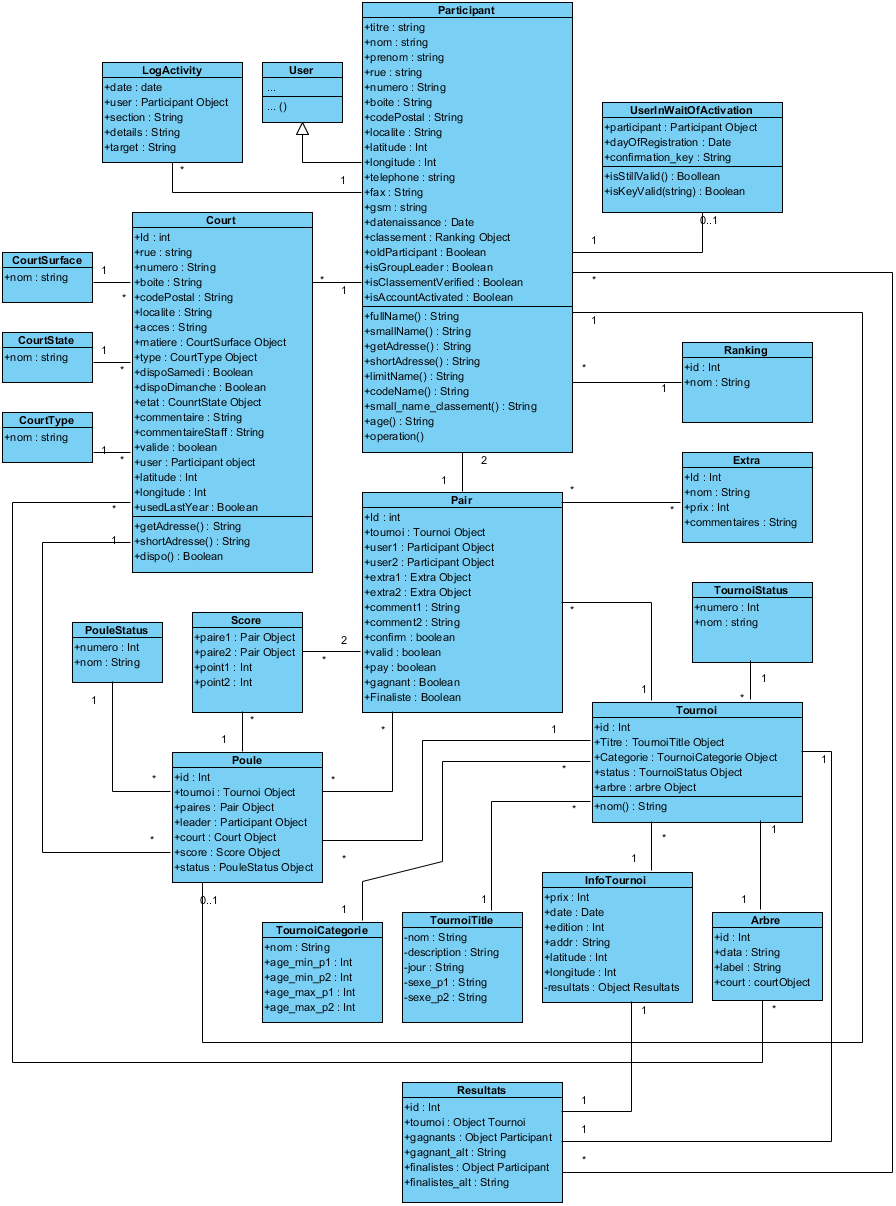
\includegraphics[width=1\linewidth]{class_dia.png}
	\caption{Class diagram of our current implementation}
	\label{fig:length_eight_mouse}
\end{figure}
\FloatBarrier
